\documentclass{beamer}
\usepackage{amsmath}
\usepackage[english]{babel} %set language; note: after changing this, you need to delete all auxiliary files to recompile
\usepackage[utf8]{inputenc} %define file encoding; latin1 is the other often used option
\usepackage{csquotes} % provides context sensitive quotation facilities
\usepackage{graphicx} %allows for inserting figures
\usepackage{booktabs} % for table formatting without vertical lines
\usepackage{textcomp} % allow for example using the Euro sign with \texteuro
\usepackage{stackengine}
\usepackage{wasysym}
\usepackage{tikzsymbols}
\usepackage{textcomp}
\usepackage{xcolor}
\usepackage[table]{xcolor}
\usepackage[dvipsnames]{xcolor}
% ELIMINAR COMANDOS DE NAVEGACION%%%%%%%%%%%
\setbeamertemplate{navigation symbols}

%\newcommand{\bubblethis}[2]{
 %       \tikz[remember picture,baseline]{\node[anchor=base,inner sep=0,outer sep=0]%
 %       (#1) {\underline{#1}};\node[overlay,cloud callout,callout relative pointer={(0.2cm,-0.7cm)},%
 %       aspect=2.5,fill=yellow!90] at ($(#1.north)+(-0.5cm,1.6cm)$) {#2};}%
 %   }%
%\tikzset{face/.style={shape=circle,minimum size=4ex,shading=radial,outer sep=0pt,
 %       inner color=white!50!yellow,outer color= yellow!70!orange}}

%% Some commands to make the code easier
\newcommand{\emoticon}[1][]{%
  \node[face,#1] (emoticon) {};
  %% The eyes are fixed.
  \draw[fill=white] (-1ex,0ex) ..controls (-0.5ex,0.2ex)and(0.5ex,0.2ex)..
        (1ex,0.0ex) ..controls ( 1.5ex,1.5ex)and( 0.2ex,1.7ex)..
        (0ex,0.4ex) ..controls (-0.2ex,1.7ex)and(-1.5ex,1.5ex)..
        (-1ex,0ex)--cycle;}
\newcommand{\pupils}{
  %% standard pupils
  \fill[shift={(0.5ex,0.5ex)},rotate=80] 
       (0,0) ellipse (0.3ex and 0.15ex);
  \fill[shift={(-0.5ex,0.5ex)},rotate=100] 
       (0,0) ellipse (0.3ex and 0.15ex);}

\newcommand{\emoticonname}[1]{
  \node[below=1ex of emoticon,font=\footnotesize,
        minimum width=4cm]{#1};}
\usepackage{scalerel}
\usetikzlibrary{positioning}
\usepackage{xcolor,amssymb}
\newcommand\dangersignb[1][2ex]{%
  \scaleto{\stackengine{0.3pt}{\scalebox{1.1}[.9]{%
  \color{red}$\blacktriangle$}}{\tiny\bfseries !}{O}{c}{F}{F}{L}}{#1}%
}
\newcommand\dangersignw[1][2ex]{%
  \scaleto{\stackengine{0.3pt}{\scalebox{1.1}[.9]{%
  \color{red}$\blacktriangle$}}{\color{white}\tiny\bfseries !}{O}{c}{F}{F}{L}}{#1}%
}
\usepackage{fontawesome} % Social Icons
\usepackage{epstopdf} % allow embedding eps-figures
\usepackage{tikz} % allows drawing figures
\usepackage{amsmath,amssymb,amsthm} %advanced math facilities
\usepackage{lmodern} %uses font that support italic and bold at the same time

\usepackage{tikz}

\usepackage{tcolorbox}

\usefonttheme[onlymath]{serif} %set math font to serif ones

\definecolor{beamerblue}{rgb}{0.2,0.2,0.7} %define beamerblue color for later use

%%% defines highlight command to set text blue
\newcommand{\highlight}[1]{{\color{blue}{#1}}}


%%%%%%% commands defining backup slides so that frame numbering is correct

\newcommand{\backupbegin}{
   \newcounter{framenumberappendix}
   \setcounter{framenumberappendix}{\value{framenumber}}
}
\newcommand{\backupend}{
   \addtocounter{framenumberappendix}{-\value{framenumber}}
   \addtocounter{framenumber}{\value{framenumberappendix}}
}

\newtcolorbox{boxA}{
    fontupper = \bf,
    boxrule = 1.5pt,
    colframe = black % frame color
}
\newtcolorbox{boxB}{
    boxrule = 1.5pt,
    colframe = blue!70!black,, % frame color
    colback = blue!7!white,
}
\usepackage{hyperref}

%%%% end of defining backup slides

%Specify figure caption, see also http://tex.stackexchange.com/questions/155738/caption-package-not-working-with-beamer
\setbeamertemplate{caption}{\insertcaption} %redefines caption to remove label "Figure".
%\setbeamerfont{caption}{size=\scriptsize,shape=\itshape,series=\bfseries} %sets figure  caption bold and italic and makes it smaller


\usetheme{Boadilla}

% --------------------
% Overall information
% --------------------
\title[Economía I]{Economía I \vspace{4mm}
\\ Magistral 5: Dentro de la firma}
\date{}
\author[Riottini]{Franco Riottini}
\vspace{0.4cm}
\institute[]{Universidad de San Andrés} 


\begin{document}

\begin{frame}
\titlepage
\centering

\includegraphics[scale=0.2]{../Figures/logoUDESA.jpg} 
\end{frame}

\begin{frame}{El comportamiento de la firma}
    \begin{itemize}
        \item ¿Cuál es el objetivo de las empresas? \vspace{2mm}
        \begin{center}
            ¡GANAR DINERO!
        \end{center}  \vspace{2mm}
         \item Seguramente los empresarios tienen otros objetivos, pero quizás los satisfacen usando parte de sus ganancias. 
         \item Las empresas que no buscan ganar dinero van a tener problemas para sobrevivir 
        \item Las decisiones que toman las empresas dependen de 
        \begin{itemize}
            \item las características del mercado (la demanda) y
            \item los costos de producción, 
            \item pero las políticas gubernamentales (por ejemplo impuestos) van a afectar también las decisiones
        \end{itemize}    
    \end{itemize}    
    \end{frame}

\begin{frame}{Restricciones y decisiones}
    \begin{itemize}
        \item Las decisiones que toma una empresa dependen de tres aspectos:
            \begin{itemize} 
            \item \textcolor{blue}{La demanda del mercado}: ¿qué es lo que los consumidores están dispuestos a comprar? ¿y a qué precios?
            \item  \textcolor{blue}{Las características del mercado}: ¿cómo se comportan las otras empresas? ¿hay muchos competidores?
            \item  \textcolor{blue}{Sus capacidades tecnológicas}: las características de su función de producción dada por sus costos de producción  \vspace{2mm}
            \end{itemize}
        \item Una empresa debe adaptarse a las dos primeras restricciones (no las puede cambiar), pero la última sí depende ella.  \vspace{2mm}
        \item Tomando en cuenta estas restricciones, la empresa toma decisiones sobre:
        \begin{itemize}
            \item el precio al que ofrece sus productos...
            \item ... y la cantidad de este producto que va a producir
        \end{itemize}
    \end{itemize} 
    \end{frame}

\begin{frame}
    \frametitle{El problema de la firma}
    \begin{itemize}
        \item Si conocemos la demanda... ¿cómo se elige cuánto producir y qué precio cobrar?
        \vspace{2mm}
        \item El problema principal de la empresa es la maximización del beneficio \vspace{2mm} 
            \begin{itemize}
            \item ¿Qué es el beneficio? \vspace{2mm}  
                \begin{center}
                Beneficio = Ingresos \ Totales - Costos \ Totales \\  \vspace{2mm}
                $\Pi = IT - CT $ 
                \end{center}
                \vspace{2mm}
            \item ¿Qué es el ingreso total?  
            El valor de la producción al precio ofrecido \\ \vspace{1mm} 
                \begin{center}
                $IT = p \cdot q$
                \end{center}
            \vspace{2mm}
            \item ¿Qué es el costo total?
            Los costos por unidad, por la cantidad de unidades producidas \\ \vspace{1mm} 
                \begin{center}
                $CT = c \cdot q$
                \end{center}
        \end{itemize} 
    \end{itemize} 
\end{frame}

\begin{frame}
\frametitle{Pensemos el ejemplo de una pizzería}
\centering

\includegraphics[scale=0.25]{../Figures/pizzeria.jpeg}
\end{frame}
        
\begin{frame}
    \frametitle{Pensando en los costos}
    \begin{itemize}
        \item Costos explícitos \vspace{2mm} 
        \begin{itemize}
            \item Harina, levadura, sal, agua, etc.
            \item Alquiler del negocio (podríamos ser los dueños pero en ese caso...)
            \item Salario de los empleados 
            \item Servicios que hay que pagar (agua, luz, gas, etc.) \vspace{2mm} 
        \end{itemize}
        \item Costos implícitos \vspace{2mm} 
        \begin{itemize}
            \item El salario que perdemos por la actividad alternativa
            \item El costo del capital invertido (que podría ser utilizado en otra actividad económica)
        \end{itemize}
    \end{itemize}
\end{frame}

\begin{frame}{Beneficio Económico vs Beneficio Contable}
    \begin{itemize}
        \item El beneficio contable es la diferencia entre los ingresos obtenidos y los gastos incurridos. \vspace{2mm} 
        \item El beneficio económico incluye los costos de oportunidad. Por lo tanto, nos dice si el negocio es rentable respecto de la siguiente mejor alternativa. \vspace{2mm} 
        \item ¿En qué piensan los contadores? En el \textbf{beneficio contable} \vspace{2mm} 
        \item ¿En qué piensan los economistas? En el \textbf{beneficio económico} \vspace{2mm} 
    \end{itemize}
\end{frame}

\begin{frame}
    \frametitle{Alta ganancia contable, baja ganancia económica}
    \centering
    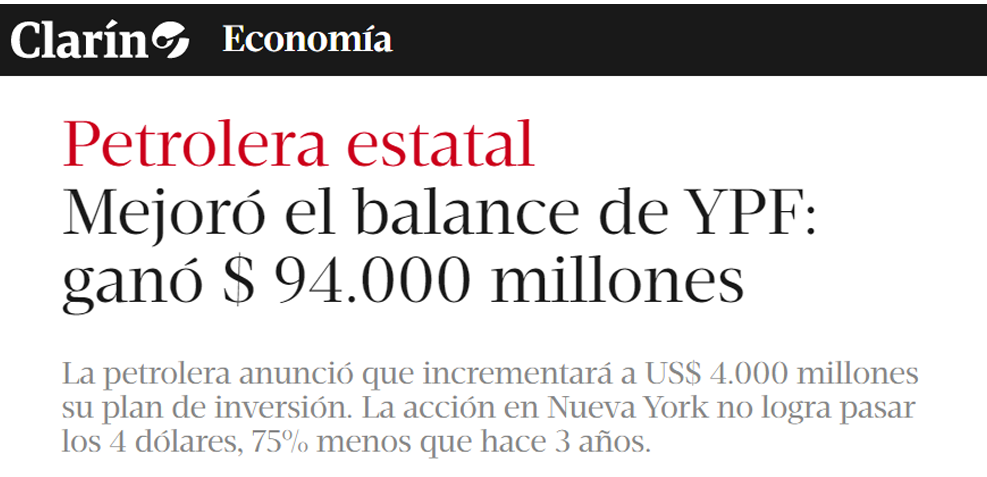
\includegraphics[scale=0.5]{../Figures/YPF.png}
\end{frame}

\begin{frame}{Regla de decisión básica}

    \begin{itemize}
        \item Para tomar una decisión, las empresas van a utilizar el análisis marginal $\Rightarrow$ tener en cuenta beneficios y costos de producir una unidad más.
        \item \textbf{Beneficio económico marginal}: cómo cambia el beneficio total de la empresa cuando cambia la cantidad producida: \\
        \[
        BMg = \frac{\Pi_1 - \Pi_0}{Q_1 - Q_0}.
        \]
        \item La regla de decisión básica es que la empresa va a producir hasta el punto en el que el beneficio económico marginal sea cero.
    \end{itemize}
\end{frame}

\begin{frame}{Regla de decisión básica}
\begin{itemize}
\item Esto es comparar ingreso marginal ($IMg$) con costo marginal ($CMg$): 
        \[
        BMg = IMg - CMg
        \]
        \item ¿Qué es el \textbf{ingreso marginal}? El ingreso total adicional que se obtiene de vender una unidad más
        \item ¿Qué es el \textbf{costo marginal}? El costo total adicional en que se incurre cuando deseamos producir una unidad adicional
        \item ¿Qué pasa si $IMg > CMg$? La empresa puede aumentar su beneficio produciendo más.
        \item ¿Qué pasa si $IMg < CMg$? La empresa puede aumentar su beneficio produciendo menos.
    \end{itemize}
    \begin{boxB}
        \begin{center}
            Las empresas producen hasta el punto en el que el costo marginal se iguala al ingreso marginal, donde se maximiza el beneficio
        \end{center}
    \end{boxB}
\end{frame}

\begin{frame}{La función de producción}
    \begin{boxA}
        \begin{center}
            La función de producción es una expresión matemática que indica la cantidad máxima de bienes que una empresa puede producir, dada su tecnología, a partir de la combinación una cantidad específica de insumos.
        \end{center}
    \end{boxA}
    Vamos a diferenciar entre el corto y el largo plazo:
    \begin{itemize}
        \item En el corto plazo puedo solo cambiar la cantidad de algunos insumos
        \begin{itemize}
            \item En el ejemplo clásico donde tengo Trabajo y Capital, puedo cambiar la cantidad de trabajo pero no la de capital
        \end{itemize}
        \item En el largo plazo puedo cambiar la cantidad de todos los insumos
        \begin{itemize}
            \item Ahora también podría cambiar la cantidad de capital, adquiriendo más maquinarias o alquilando nuevos lugares, entre muchos otros ejemplos
        \end{itemize}
    \end{itemize}
\end{frame}

\begin{frame}
\frametitle{La función de producción en el corto plazo...}
\centering
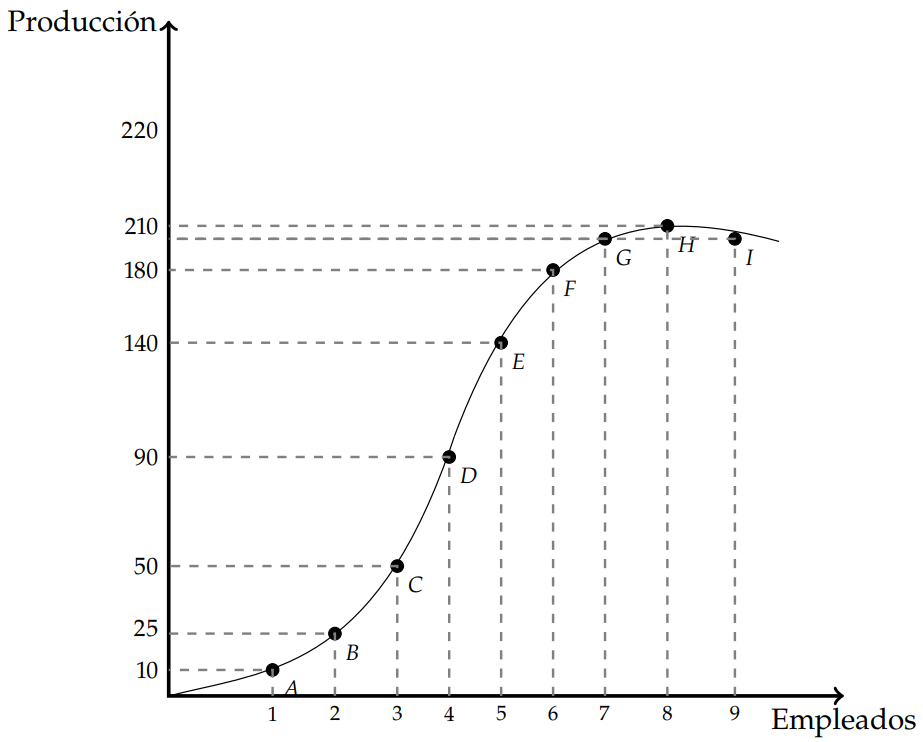
\includegraphics[scale=0.5]{../Figures/C12.1.png}
\end{frame}

\begin{frame}
    \frametitle{Contratando a un empleado adicional}
    \begin{itemize}
        \item Si observamos la función de producción anterior, la cantidad de producción que suma cada trabajador adicicional es distinta dependiendo cuantos trabajadores ya tengo
        \item Esto quiere decir que lo que cambia a medida que contrato más trabajadores es el \textbf{producto marginal}
        \item El producto marginal es la cantidad de producción adicional que se genera al aumentar la cantidad de trabajadores en una unidad
        \[ PMg = \frac{\Delta Q}{\Delta L} \]
        \item Además, esto va a cambiar el \textbf{producto medio}\dots
        \item El producto medio representa la cantidad de producto que cada trabajador genera en promedio (durante un periodo de tiempo dado)
        \[ PMe = \frac{Q}{L} \]
    \end{itemize}
\end{frame}

\begin{frame}
    \frametitle{Producto marginal y medio}
    \begin{table}[h]
        \centering
        \begin{minipage}{0.45\textwidth}
        \renewcommand{\arraystretch}{1.3}
        \small
        \begin{tabular}{cccc}
            \hline
            \textbf{L} & \textbf{Producción} & \textbf{PMe} & \textbf{PMg} \\
            \hline
            1 & 10  & 10    &    \\
            2 & 25  & 12.5  & 15 \\
            3 & 50  & 16.66 & 25 \\
            4 & 90  & 22.5  & 40 \\
            5 & 140 & 28    & 50 \\
            6 & 180 & 30    & 40 \\
            7 & 210 & 30    & 30 \\
            8 & 220 & 27.5  & 10 \\
            9 & 210 & 23.33 & -10 \\
            \hline
        \end{tabular}
        \end{minipage}
        \begin{minipage}{0.45\textwidth}
            \centering
            \vspace{11mm}
            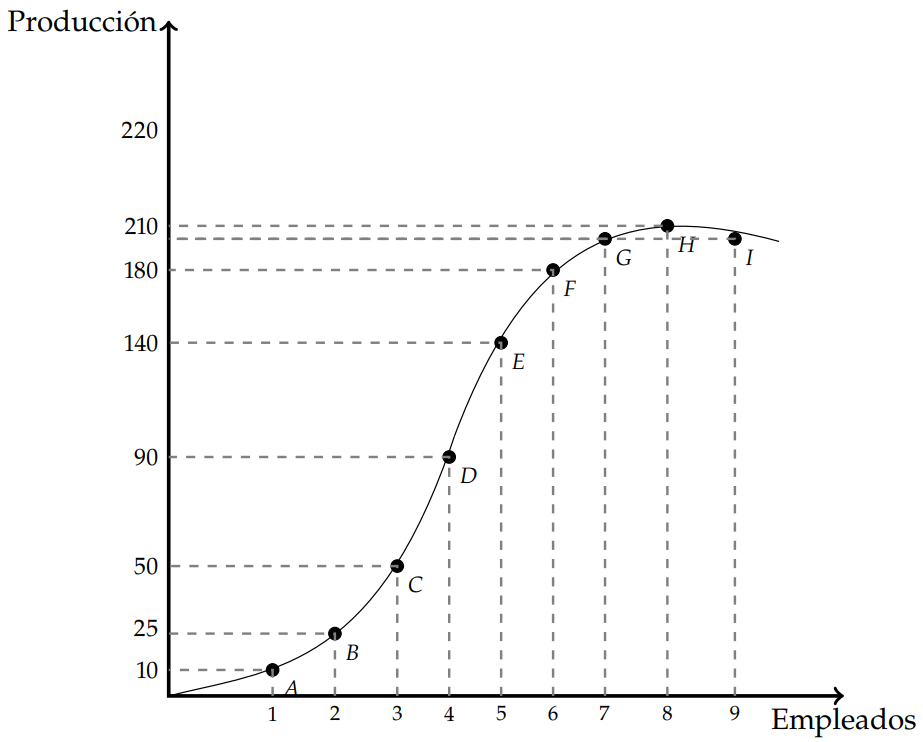
\includegraphics[scale=0.3]{../Figures/C12.1.png} 
        \end{minipage}
    \end{table}
    \end{frame}

\begin{frame}
    \frametitle{Producto marginal y medio}
    \centering
    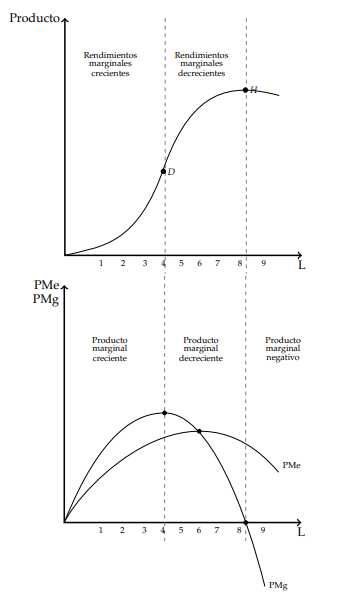
\includegraphics[scale=0.65]{../Figures/C12.7.png}
\end{frame}

\begin{frame}{Producción y costos}
\begin{itemize}
    \item La función de producción puede verse también como una función de costos
    \item ¿Por qué? Porque los costos de producción están intrinsecamente relacionados con la cantidad de producción
    \item Por ende, el producto marginal va a estar muy relacionado con el costo marginal
    \item Los costos son de dos tipos
    \begin{itemize} 
        \item Los costos fijos (no cambian con la producción)
        \item Los costos variables (cambian con la producción)
    \end{itemize}
    \item En largo plazo, vamos a asumir que todos los costos cambian con el nivel de producción\dots
    \item Si esto pasa, no hay costos fijos en el largo plazo!
\end{itemize}
\end{frame}

\begin{frame}{Veamos los costos fijos...}
    \begin{center}
        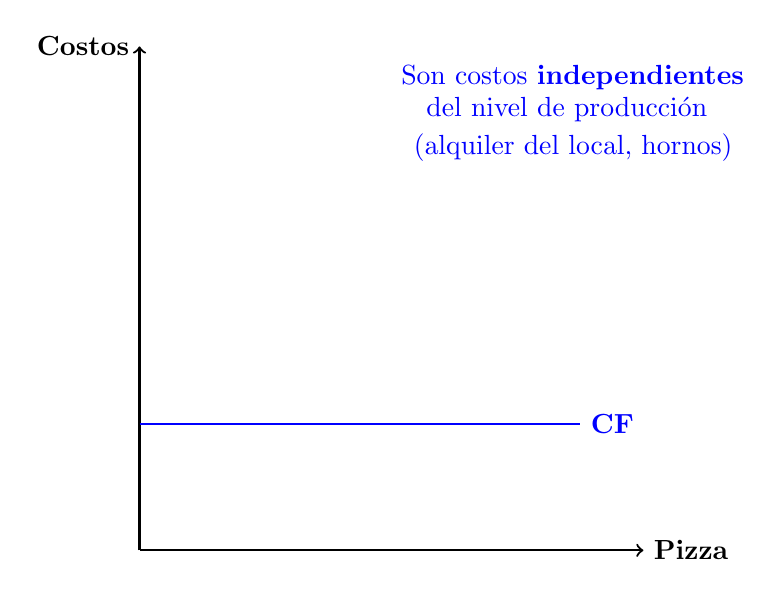
\begin{tikzpicture}[scale=0.8]
            % Ejes
            \draw[thick,->] (0,0) -- (8,0) node[right] {\textbf{Pizza}};
            \draw[thick,->] (0,0) -- (0,8) node[left] {\textbf{Costos}};
    
            % Curvas de costos
            %\draw[thick] (0,2) to[out=60,in=180] (3,4.5) to[out=0,in=250] (7,7.5) node[right] {\textbf{CT}};
            
            %\draw[thick] (0,0) to[out=60,in=180] (3,2.5) to[out=0,in=250] (7,5) node[right] {\textbf{CV}};
            
            \draw[thick, Blue] (0,2) -- (7,2) node[right] 
            {\textbf{CF}};
    
            \node[right, Blue] at (4,7.5) {Son costos \textbf{independientes}};
            \node[right, Blue] at (4.4,7) {del nivel de producción};
            
            \node[right, Blue] at (4.2,6.4) {(alquiler del local, hornos)};
        \end{tikzpicture}
    \end{center}
\end{frame}

\begin{frame}{y ahora los costos variables}
\begin{center}
    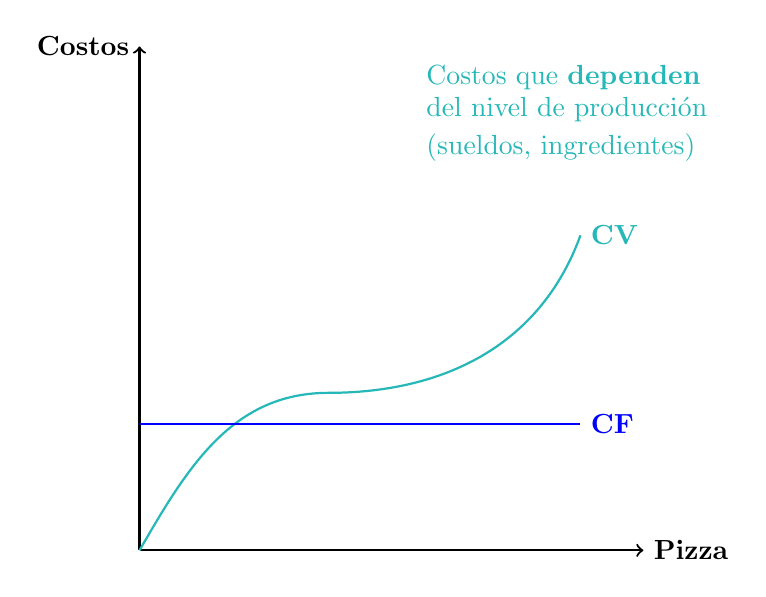
\begin{tikzpicture}[scale=0.8]
        % Ejes
        \draw[thick,->] (0,0) -- (8,0) node[right] {\textbf{Pizza}};
        \draw[thick,->] (0,0) -- (0,8) node[left] {\textbf{Costos}};

        % Curvas de costos
        %\draw[thick] (0,2) to[out=60,in=180] (3,4.5) to[out=0,in=250] (7,7.5) node[right] {\textbf{CT}};
        
        \draw[thick, BlueGreen] (0,0) to[out=60,in=180] (3,2.5) to[out=0,in=250] (7,5) node[right] {\textbf{CV}};
        
        \draw[thick, Blue] (0,2) -- (7,2) node[right] 
        {\textbf{CF}};

        \node[right, BlueGreen] at (4.4,7.5) {Costos que \textbf{dependen}};
        \node[right, BlueGreen] at (4.4,7) {del nivel de producción};
        \node[right, BlueGreen] at (4.4,6.4) {(sueldos, ingredientes)};

    \end{tikzpicture}
\end{center}
\end{frame}

\begin{frame}{Los costos totales}
    \begin{center}
        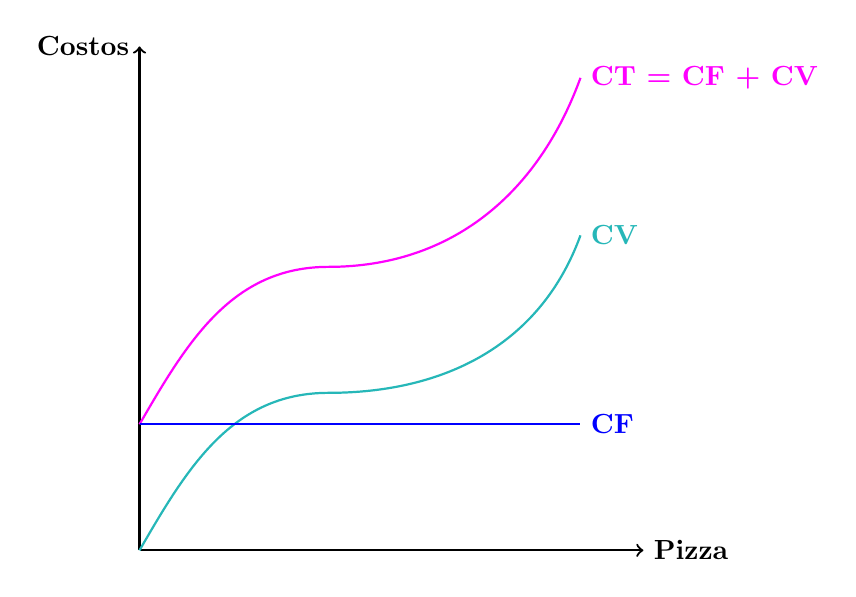
\begin{tikzpicture}[scale=0.8]
            % Ejes
            \draw[thick,->] (0,0) -- (8,0) node[right] {\textbf{Pizza}};
            \draw[thick,->] (0,0) -- (0,8) node[left] {\textbf{Costos}};
    
            % Curvas de costos
            \draw[thick, Fuchsia] (0,2) to[out=60,in=180] (3,4.5) to[out=0,in=250] (7,7.5) node[right] {\textbf{CT = CF + CV}};
            
            \draw[thick, BlueGreen] (0,0) to[out=60,in=180] (3,2.5) to[out=0,in=250] (7,5) node[right] {\textbf{CV}};
            
            \draw[thick, Blue] (0,2) -- (7,2) node[right] 
            {\textbf{CF}};
    
        \end{tikzpicture}
    \end{center}
\end{frame}

\begin{frame}
\frametitle{Los costos de hacer pizzas}
\begin{itemize}
    \item Se observan dos tipos de costos: 
        \begin{itemize}
        \item Los costos fijos
        \item Los costos variables
        \end{itemize}
    \vspace{2mm}
    \item Para evaluar la cantidad de pizzas que queremos producir nos vamos a hacer dos preguntas:
        \begin{itemize}
        \item ¿Cuánto cuesta en promedio una pizza? (Costo medio)
        \item ¿Cuánto cuesta hacer una pizza adicional? (Costo marginal)
        \end{itemize}
\end{itemize}
\end{frame}

\begin{frame}{Los costos medios}
    \begin{minipage}{0.45\textwidth}
            \begin{itemize}
            \item El costo medio es el costo promedio de una unidad producida:
                \[ CTMe = \frac{CT}{Q} \]
            \item Gráficamente es la pendiente del rayo que sale desde el origen a un punto dado de la función de costo. 
            \item También podemos calcular los otros costos medios:
            \[
            CVMe = \frac{CV}{Q} \quad CFMe = \frac{CF}{Q}
            \]
            \end{itemize}
    \end{minipage}
    \hfill
    \begin{minipage}{0.4\textwidth}
    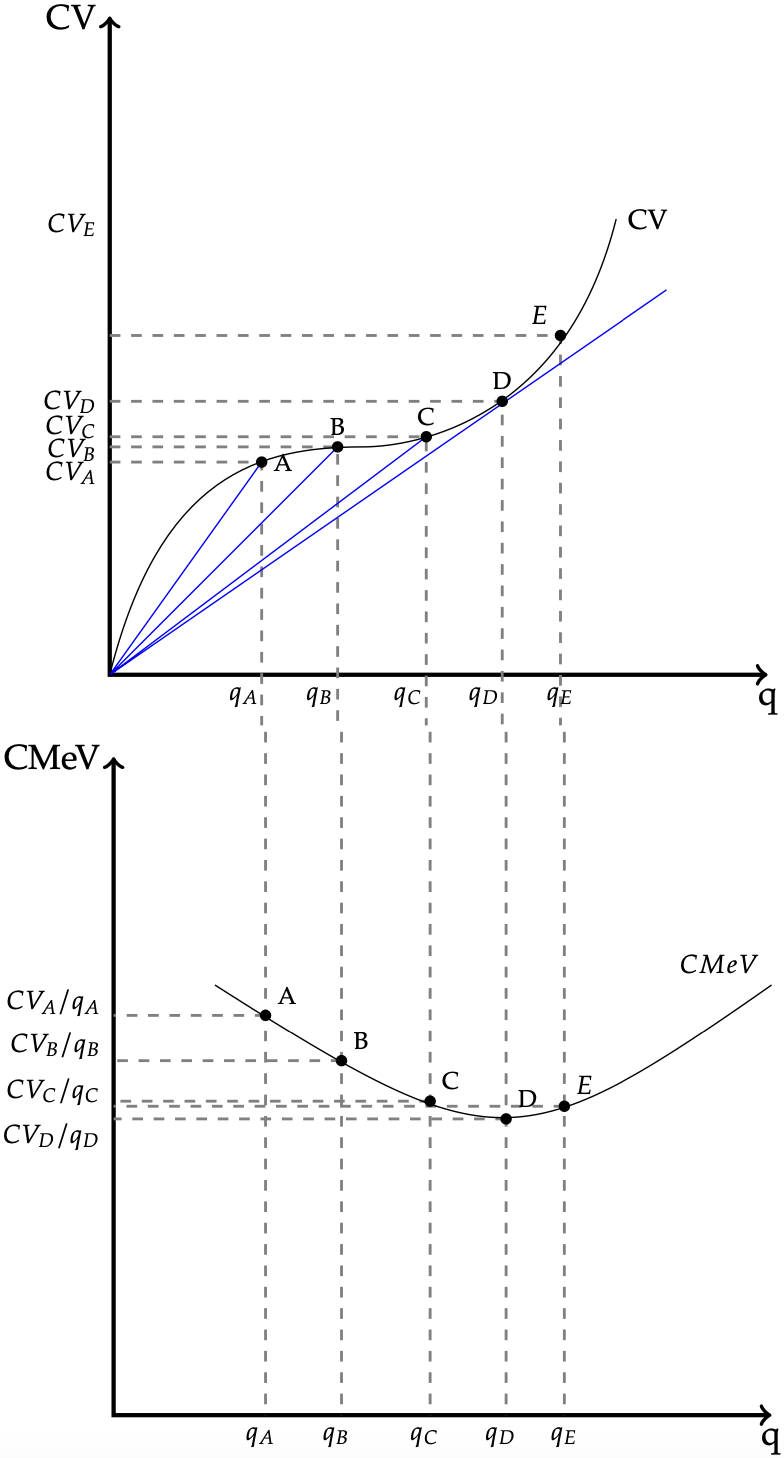
\includegraphics[scale=0.31]{../Figures/C13.5.png}
    \end{minipage}
\end{frame}

    
\begin{frame}
\frametitle{Los costos marginales}
    \begin{minipage}{0.5\textwidth}
    \begin{itemize}
    \item El costo marginal es el costo adicional que enfrenta la empresa al aumentar la producción en una unidad 
        \[ CMg = \frac{\Delta CT}{\Delta Q} = \frac{CT_1 - CT_0}{q_1 - q_0} \]
    \item Gráficamente, es la pendiente de la recta tangente en cada punto de la curva de costo total
    \end{itemize}
    \end{minipage}
    \hfill
    \begin{minipage}{0.4\textwidth}
    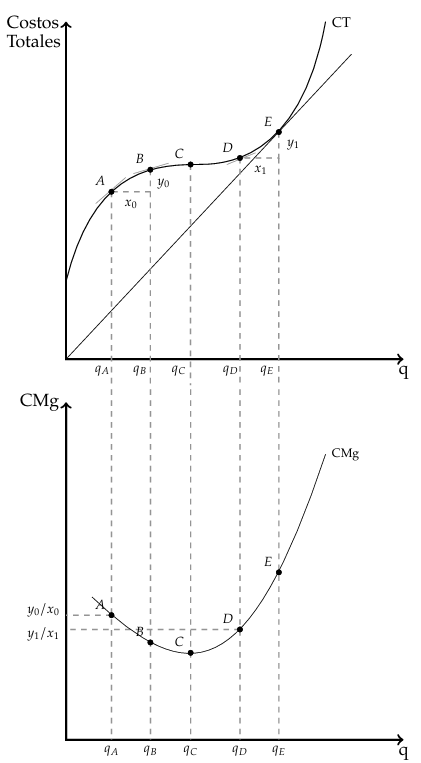
\includegraphics[scale=0.31]{../Figures/C13.7.png}
    \end{minipage}
\end{frame}

\begin{frame}{Costos: ¡para completar! }
    \begin{table}[h]
        \centering
        \renewcommand{\arraystretch}{1.5} % Espaciado entre filas
        \setlength{\tabcolsep}{6pt} % Espaciado entre columnas
        \rowcolors{2}{white!100}{white!95} % Alternar colores de filas
        \newcolumntype{P}{>{\centering\arraybackslash}p{1cm}}
        \begin{tabular}{|P|P|P|P|P|P|P|P|}
            \hline
            \rowcolor{blue!20} % Color de fondo del encabezado
            \textbf{Q} & \textbf{CF} & \textbf{CV} & \textbf{CT} & \textbf{CMg} & \textbf{CFMe} & \textbf{CVMe} & \textbf{CTMe} \\
            \hline
            0 & 40 & 0   &    & -   & -  & -  &  - \\
            1 & 40 & 20  &    &    &    &    &    \\
            2 & 40 & 35  &    &    &    &    &    \\
            3 & 40 & 45  &    &    &    &    &    \\
            4 & 40 & 65  &    &    &    &    &    \\
            5 & 40 & 100 &    &    &    &    &    \\
            \hline
        \end{tabular}
    \end{table}
\end{frame}

\begin{frame}{¿Cómo construir los costos medios?}
\centering
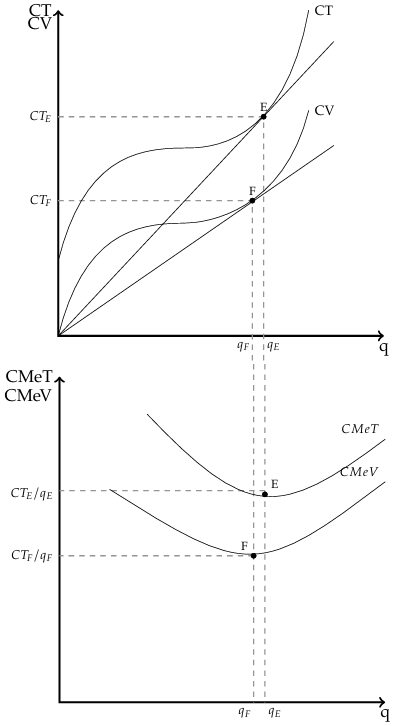
\includegraphics[scale=0.5]{../Figures/C13.6.png}
\end{frame}

\begin{frame}
\frametitle{¿Cómo construir el costo marginal?}
\centering
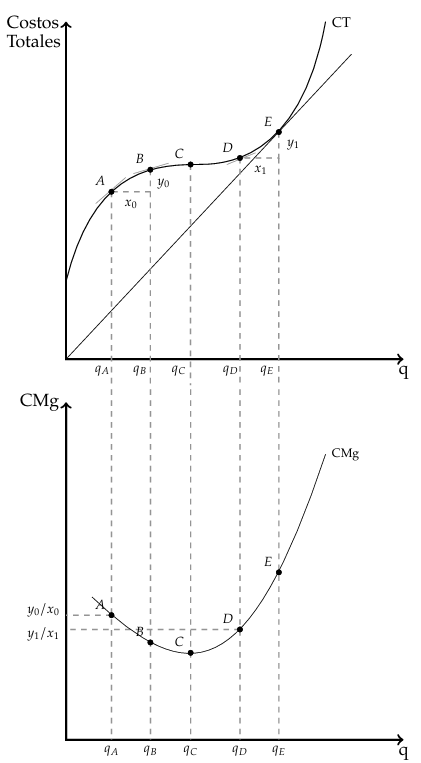
\includegraphics[scale=0.5]{../Figures/C13.7.png}
\end{frame}

\begin{frame}
\frametitle{Graficando costo medio y marginal en el mismo gráfico}
\centering
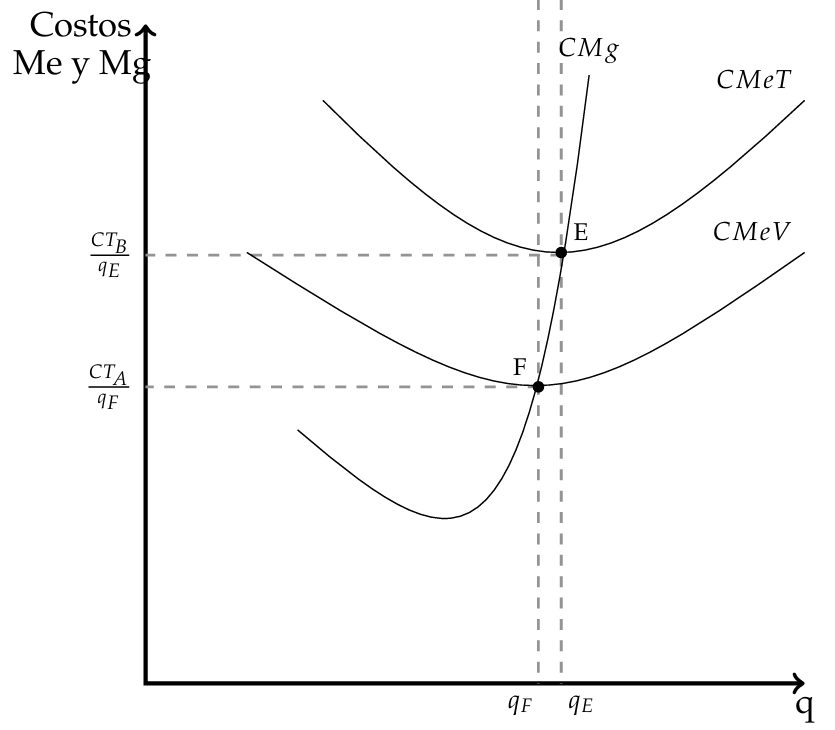
\includegraphics[scale=0.45]{../Figures/C13.8.png}
\end{frame}

\begin{frame}
\frametitle{Las propiedades de las curvas}
\begin{itemize}
    \item El costo marginal eventualmente aumenta debido a los rendimientos marginales decrecientes.
    \item La curva de costo total promedio suele tener forma de U. Bajan los costos fijos medios y aumentan los costos variables medios.
    \item La curva de costo marginal corta la curva de costo total promedio en su nivel mínimo.
    \item Si el costo marginal es menor al costo medio, el costo medio disminuye al aumentarla producción
\end{itemize}
\end{frame}


\end{document}